\chapter{Introduction}

\begin{bibunit}

\section{Fundamental Physics}

The discovery of the cosmic microwave background (CMB) radiation by \citet{1965ApJ...142..419P}
provided the first direct evidence that the universe had a beginning. Arno Penzias and Robert Wilson
shared the 1978 Nobel Prize in Physics for this discovery, and astronomers have been studying this
radiation ever since. In fact, a second Nobel Prize was awarded to John Mather and George Smoot in
2006 for their work on the Cosmic Background Explorer (COBE) satellite, which was amongst the first
experiments to demonstrate that the background radiation was anisotropic
\citep{1992ApJ...396L...1S}. These studies of the CMB have fundamentally advanced humanity's
understanding of the universe: its origin, evolution, and composition. Still we continue to study
the CMB particularly because it illuminates everything in the universe. It is a flashlight for the
darkness of space within our expanding universe.

As the universe expands, the wavelength of a photon is similarly stretched or redshifted (so-called
because it gradually drifts to longer, redder wavelengths). Photons originating from a star 1000
light-years away will travel through the universe for 1000 years before they are collected by our
telescopes. Consequently, we observe this star as it was 1000 years ago. However, during its travels,
the photon was also stretched by a small factor of $0.000007\%$ due to the expansion of the
universe.  For nearby stars, this expansion factor is clearly too small to be conceivably measured.
However, with the discovery of the first quasar by \citet{1963Natur.197.1040S} it soon became
apparent that the stretching factor, the redshift $z$, can be $>10\%$. Today, the most distant known
quasars and galaxies are so far away that the wavelength has more than doubled ($z > 1$) due to the
expansion of the universe \citep{2011Natur.474..616M, 2015ApJ...810L..12Z, 2016ApJ...819..129O,
2018Natur.553..473B}.

Due largely to careful and detailed work studying the CMB \citep[e.g.,][]{2016A&A...594A..25P}, Type
Ia supernova explosions \citep[e.g.,][]{1998AJ....116.1009R,1999ApJ...517..565P}, and cosmological
galaxy surveys \citep[e.g.,][]{2001MNRAS.328.1039C}, we have a coherent and consistent understanding
of the expansion history of the universe. The redshift $z$ is therefore commonly used as a proxy
for distance. The higher the redshift, the longer the photon has been in transit, and the further
its origin. However, in order to measure the redshift, the measured photon must originate from a
known spectral feature.

Despite its abundance, neutral hydrogen (\ion{H}{1}) has few low energy transitions that allow it to
be traced.  Due to this limitation, astronomers resort to using a hyperfine structure transition
arising from the magnetic dipole interaction between proton and electron. This interaction leads to
a slight energy difference between the spin-symmetric state and the spin-antisymmetric state. The
energy difference is $hc / (21\,\text{cm})$ where $h$ is Planck's constant, and $c$ is the speed of
light.  When a Hydrogen atom transitions from the spin-symmetric state (higher energy) to the
spin-antisymmetric state (lower energy), it emits a photon with a wavelength of $21\,\text{cm}$ or a
frequency of $1420\,\text{MHz}$. The redshift $z$ of a 21~cm photon is therefore computed from the
observed frequency $\nu$ as
\begin{equation}
    z = \frac{1420\,\text{MHz}}{\nu} - 1\,.
\end{equation}

\begin{figure}[t]
    \centering
    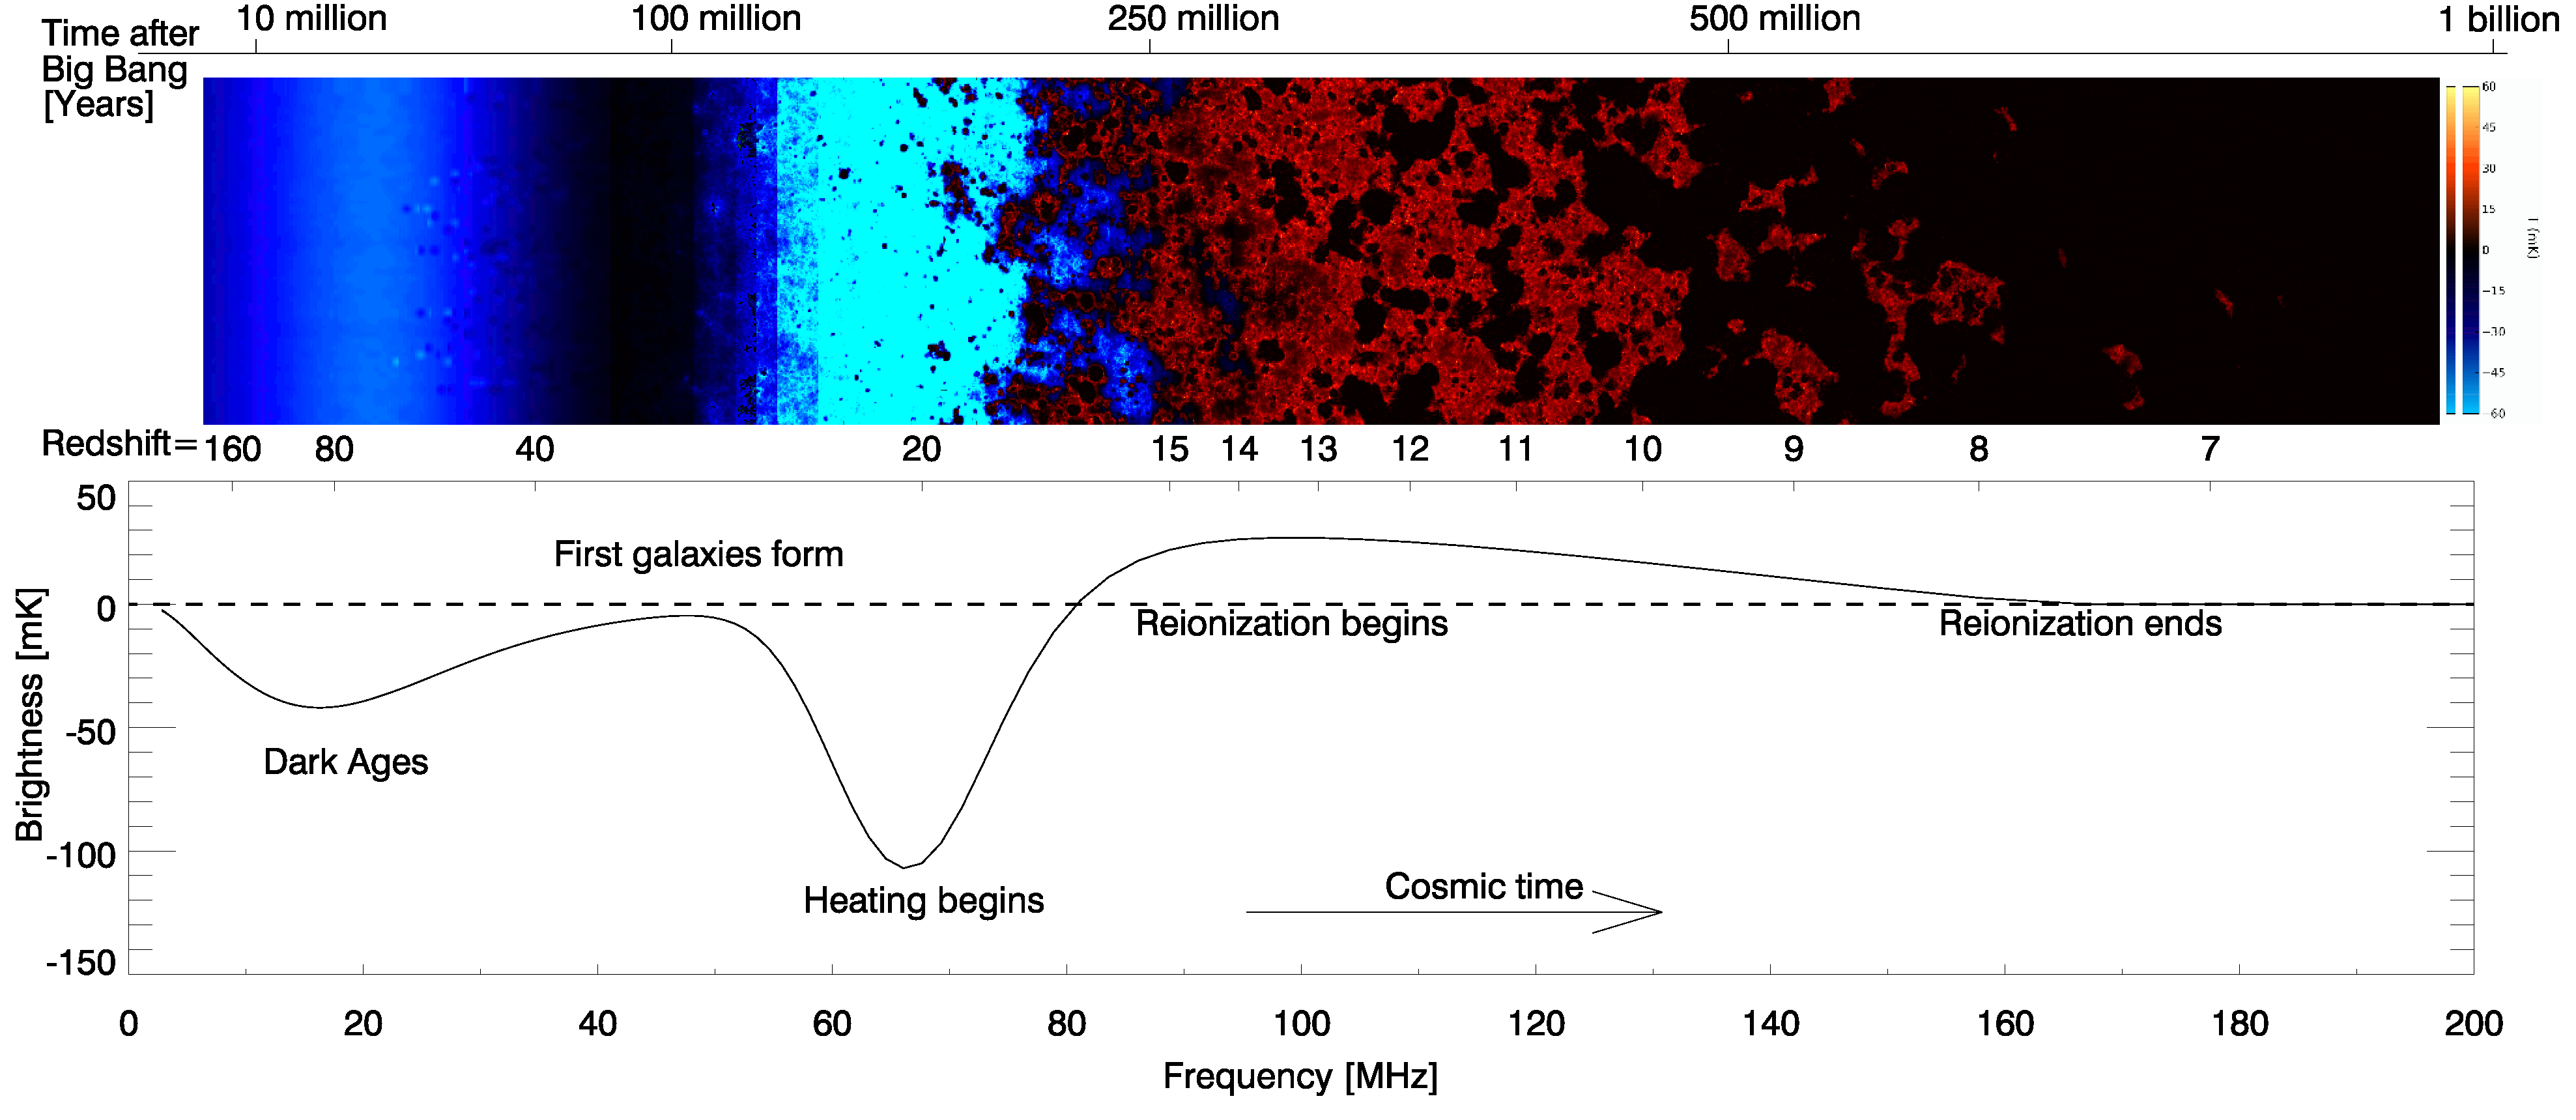
\includegraphics[width=\textwidth]{figures/chapter1/pritchard-2012-global-signal}
    \caption{
        (top) A simulated light cone of the 21~cm brightness temperature illustrating the
        anisotropy in the expected signal.
        (bottom) A simulation of the globally averaged brightness temperature due to the high
        redshift 21~cm transition.
        This figure is reproduced with permission from \citet{2012RPPh...75h6901P}.
    }
    \label{fig:pritchard-global-signal}
\end{figure}

Neutral hydrogen in the early universe is illuminated by the CMB. A calculation of the radiative
transfer \citep{2012RPPh...75h6901P} yields (neglecting the contribution of peculiar velocities):
\begin{equation}\label{eq:radiative-transfer-equation}
    \Delta T_{21} \approx 27 \left[
        \overbrace{
            x_\text{HI} (1+\delta)
            \left(\frac{\Omega_b h}{0.0327}\right)
        }^{\text{quantity of HI}}
        \left(\frac{\Omega_m}{0.307}\right)^{-1/2}
        \left(\frac{1+z}{10}\right)^{1/2}
        \overbrace{
            \left(\frac{T_\text{spin} - T_\text{CMB}(z)}{T_\text{spin}}\right)
        }^{\text{relative temperature}}
    \right] \, {\rm mK} \,,
\end{equation}
where $\Delta T_{21}$ is the expected 21~cm brightness temperature. If $\Delta T_{21} > 0$, it
appears in emission against the CMB. If $\Delta T_{21} < 0$, it appears in absorption. $x_\text{HI}$
is the neutral fraction of hydrogen, $\delta$ is the local baryon overdensity, $h$ is the Hubble
constant, $\Omega_b$ is the density parameter for baryons, $\Omega_m$ is the density parameter for
matter, $T_\text{spin}$ is the spin temperature (excitation temperature of the 21~cm transition),
and $T_\text{CMB}(z) = 2.73\,(1+z)\,{\rm K}$ is the temperature of the CMB at the redshift $z$.

Equation~\ref{eq:radiative-transfer-equation} is fundamental to determining what can be learned
through detecting the 21~cm transition at high redshift. First, if the spin temperature is greater
than the CMB temperature, the 21~cm transition appears in emission. However, the signal saturates at
high spin temperatures. If the spin temperature is less than the CMB temperature, the 21~cm
transition appears in absorption with no saturation point. Second, the amplitude of the signal is
proportional to the total quantity of \ion{H}{1}. Therefore, in order for there to be a measurable
21~cm signal, the universe must be predominantly neutral, and the transition must not be in
radiative equilibrium with the CMB. An example prediction for $\Delta T_{21}$ can be seen in
Figure~\ref{fig:pritchard-global-signal}.

There are three relevant temperatures that affect the spin temperature: $T_\text{gas}$, the
temperature of the gas, $T_\text{CMB}$, the temperature of the CMB, and $T_{\text{Ly}\alpha}$, the
color temperature of the Ly$\alpha$ radiation from early star formation. More exotic theories might
also include the temperature of the dark matter, $T_\text{DM}$. Generally,  the Ly$\alpha$ photons
scatter through the intergalactic medium (IGM), which sets $T_{\text{Ly}\alpha} = T_\text{gas}$. In
the absence of any heating mechanisms, the matter and radiation are both cooling adiabatically with
the expansion of the universe.  The adiabatic indices are $\gamma = 5/3$ and $\gamma = 4/3$
respectively, so the matter cools faster than the radiation. Consequently, the 21~cm transition
tends to appear in absorption prior to early star formation, and in emission after the IGM has been
heated.

While there are currently few observational constraints on the 21~cm brightness temperature,
fiducial theoretical models tell the following story\todo{add a reference here}.  During the dark
ages ($z \gtrsim 40$) the density of the universe is high enough for collisions between hydrogen
atoms to dominate the excitation of the 21~cm transition.  Consequently during this time
$T_\text{spin} = T_\text{gas}$, and the 21~cm transition appears in absorption against the CMB.
Later ($z \sim 30$), as the mean density of the universe decreases, collisions become more
infrequent and the 21~cm transition is instead excited by CMB photons. During this time the 21~cm
signal vanishes because $T_\text{spin} = T_\text{CMB}$.

With the onset of star formation in the universe, the IGM is inundated with Ly$\alpha$ photons.
These Ly$\alpha$ photons scatter through the IGM. With the absorption and re-emission of a
Ly$\alpha$ photon, a hydrogen atom can transition between the spin-symmetric state and the
spin-antisymmetric state. This process, called the Wouthuysen-Field effect, sets the relative
abundance of \ion{H}{1} in each state such that $T_\text{spin} = T_{\text{Ly}\alpha} = T_\text{gas}$
\citep{1952AJ.....57R..31W,1958PIRE...46..240F}. Therefore, after early star formation begins, the
21~cm transition reappears in absorption against the CMB.

However, as star formation progresses, the gas in the IGM is heated. X-rays are particularly
effective at heating the IGM due to their large mean-free path. Consequently the heating rate is
sensitive to, for example, the number density, luminosity and spectral hardness of X-ray binaries.
Eventually the gas is heated above the temperature of the CMB, bringing the 21~cm transition into
emission, and eventually the signal saturates. At this point the 21~cm
transition begins to disappear with the onset of reionization at $z \lesssim 15$ due to the
disappearance of neutral hydrogen. A prediction of the spectral distortion this process applies to
the low-frequency ($\nu < 200\,\text{MHz}$) CMB spectrum can be seen in the bottom panel of
Figure~\ref{fig:pritchard-global-signal}.









For much of the universe's history, the intergalactic medium (IGM) is ionized or in radiative
equilibrium with the CMB.





Given knowledge of the
original wavelength of the photon, and the expansion history of the universe, we can calculate how
long the photon must have been in flight.


Today the CMB is a 2.7\,K sea of photons that permeates the universe. This radiation is constantly
cooling due to the inexorable expansion of the universe.

\todo{more context of other high-z probes of the universe}

\todo{talk about Tzu-Ching's detection}


\section{First Generation Experiments}

Ultimately, it may be possible to map the EoR and cosmic dawn through the 21\,cm line
\citep{1997ApJ...475..429M}. In fact, this is called a ``main science goal'' for the future Square
Kilometer Array \citep[SKA;][]{2013ExA....36..235M}.  First generation experiments, however, are of
somewhat more limited scope and therefore employ statistical averages to boost sensitivity to the
high-redshift 21\,cm signal.

The two most popular statistics are the global average and the power spectrum. The global average or
monopole averages over all lines of sight, mapping the 21\,cm brightness temperature within
spherical shells of the universe:
\begin{equation}
    T^\text{global}_{21}(z) = \frac{1}{\Omega}\int \Delta T_{21}(\vec{r}) \, \d\Omega \,,
\end{equation}
where $T^\text{global}_{21}(z)$ is the global 21\,cm signal at the redshift $z$, $\Delta
T_{21}(\vec{r})$ is the 21\,cm brightness temperature at the position $\vec{r}$, and the integral
runs over solid angle $\Omega$.  The power spectrum statistic leverages the line of sight distance
information from the observed frequency to measure the power in fluctuations on a given spatial
scale within a volume of the universe:
\begin{equation}
    P_{21}(z; \vec{k}) =
        \frac{1}{V}\left|
        \int \Delta T_{21}(\vec{r}) \, e^{-i\vec{k}\cdot\vec{r}} \, \d^3r
        \right|^2\,,
\end{equation}
where $P_{21}(z; \vec{k})$ is the three-dimensional spatial power spectrum at the redshift $z$ and
wavevector $\vec{k})$, and the integral runs over the observed volume $V$ of the universe.
Neglecting redshift-space distortions, the spatial power spectrum of 21\,cm fluctuations is expected
to be isotropic. Therefore, typically the power spectrum $P(\vec{k})$ is averaged over the
orientation of the wavevector $\vec{k}$. Instrumental considerations typically lead to different
sources of systematic errors along the line of sight and perpendicular to the line of sight, so
parameterizing the power spectrum in terms of the parallel and perpendicular to the line of sight
wavenumbers ($k_\parallel$ and $k_\perp$ respectively) is common.

The global signal and the power spectrum are both statistics of the same underlying 21\,cm
brightness temperature and therefore statistics can be used to answer high-level questions such as:
When did reionization occur? How quickly was the universe heated after initial star formation began?
The power spectrum contains additional information about sources of heating and ionization. For
instance, rare massive haloes generate fluctuations on larger spatial scales than the more common
small haloes.  However, because measuring the power spectrum requires angular resolution, the global
signal experiments and power spectrum experiments employ substantially different instrumental
designs. They are subject to different (but not exclusively different) systematic instrumental
errors.

%Two different types of experiments are currently being designed to target the high-redshift 21~cm
%transition:
%\begin{enumerate}
%    \item single antenna experiments that are attempting to measure the sky-averaged 21~cm signal,
%        and
%    \item large interferometers that are attempting to measure the three-dimensional spatial power
%        spectrum of the 21~cm signal.
%\end{enumerate}
%Both types require exquisite calibration and roughly five orders of dynamic range against the
%blindingly bright foreground radio emission, but are subject to different (but not exclusively
%different) systematic instrumental errors.

\subsection{Global Signal Experiments}

Most global signal experiments are composed of a single dipole antenna with a total power
radiometer. This approach was pioneered by the Experiment to Detect the Global EoR Signature
(EDGES). After deploying to the Murchison Radio-astronomy Observatory (MRO) in a remote region of
Western Australia, \citet{2010Natur.468..796B} observed for three months. If reionization was an
instantaneous event, this initial EDGES deployment would have expected to see a step function in
their sky-averaged spectrum. Therefore the authors converted the observed spectral smoothness to a
lower bound on the duration of reionization $\Delta z > 0.06$. However, because no such feature was
detected, the redshift of reionization was not constrained by this measurement.

\todo{LEDA}

\todo{SARAS}

Although most global signal experiments are composed of isolated dipole antennas, there have been
several attempts to design and use more exotic instruments. \citet{2013PhRvD..87d3002L} found that
an instrument with a 5$\arcdeg$ beam could achieve a higher significance detection by using the
improved angular resolution to mitigate foreground contamination. \citet{2015MNRAS.450.2291V} used
lunar occultation to constrain the global signal between 35 and 80\,MHz using LOFAR. This technique
uses an interferometer to measure the contrast between the moon and surrounding sky, but is
complicated by radio frequency interference (RFI) reflecting off of the moon and potentially by the
assumption that the moon is a thermal source at low frequencies. Drawn by the calibration advantages
of interferometers, other groups have proposed designing interferometers that have nonzero
sensitivity to the monopole. \citet{2015ApJ...809...18P} developed a framework for measuring the
global signal from interferometric measurements, and \citet{2015ApJ...815...88S} designed a
zero-spacing interferometer using a resistive screen to separate two antennas. However, ultimately
the calibration advantages of an interferometer to measure the global signal may have been
overstated.  \citet{2016ApJ...826..116V} demonstrated that interferometers may only have any
sensitivity to the global signal if there is some amount of cross talk between the correlated
elements or a source of noise that can radiate coherently into both receivers.

\subsection{Power Spectrum Experiments}

\begin{figure}[t]
    \centering
    \includegraphics[width=\textwidth]{figures/chapter1/power-spectrum-upper-limits/power-spectrum-upper-limits}
    \caption{
        Power spectrum amplitude upper limits (95\% confidence or lowest systematically limited data
        point) as a function of redshift. The shaded region denotes roughly where current
        theoretical predictions fall.
    }
    \label{fig:power-spectrum-upper-limits}
\end{figure}

In contrast to the global signal experiments, which are typically composed of a single antenna,
power spectrum experiments are generally interferometers composed of up to hundreds or thousands of
antennas. A high-level overview of existing upper limits on the 21\,cm power spectrum can be seen in
Figure~\ref{fig:power-spectrum-upper-limits}.

\todo{GMRT}

The Donald C. Backer Precision Array for Probing the Epoch of Reionization
\citep[PAPER;][]{2010AJ....139.1468P} began attempting to measure the 21\,cm power spectrum with a
deployment of eight antennas in Green Bank, West Virginia. Later deployed with 32 antennas to the
Karoo desert in South Africa, \citet{2014ApJ...788..106P} measured a $2\sigma$ upper limit of 41\,mK
on the amplitude of the power spectrum at $z=7.7$. This measurement ruled out the possibility that
the universe was entirely unheated by this redshift.  Later, with PAPER now composed of 64 antennas,
\citet{2015ApJ...809...61A} improved the best $2\sigma$ upper limit to 22.4\,mK at $z=8.4$, however
this is result is currently subject to revision (Cheng et al. in prep.). PAPER is notable for its
decision to part with traditional interferometry. Starting with its 32-antenna deployment, PAPER
opted for a maximally redundant antenna configuration for raw sensitivity on a particular spatial
scale.

The Low-Frequency Array (LOFAR) EoR Key Science Project (KSP) is attempting a similar measurement of
the 21\,cm power spectrum. In contrast to PAPER, LOFAR is composed of $\sim30,000$ high-band
antennas (120--240\,MHz) and $\sim3,000$ low-band antennas (30--80\,MHz). These antennas are grouped
into stations and stations are correlated with each other. This trade off sacrifices field of view
for gain. The LOFAR EoR KSP recently published its first limits on the 21\,cm power spectrum,
finding a $2\sigma$ upper limit of 79.6\,mK at $z=10.1$ \citep{2017ApJ...838...65P}. In this
measurement, LOFAR attempted to leverage its superior imaging and source-removal capabilities, but
for this measurement was limited by residual systematic errors. The removal of contaminating diffuse
radio emission has been the focus of ongoing work with some reported success \citep{koopmans_2017}.

Several attempts have been made to measure the 21\,cm power spectrum with the Murchison Widefield
Array (MWA).
\todo{MWA}


\section{Observational Challenges}

Likely the most substantial challenge faced by both classes of experiments is the existence of
foreground radio emission. At large angular scales $\theta \gg 1\arcdeg$, the radio sky is dominated
by galactic synchrotron emission generated by relativistic electrons spiralling around galactic
magnetic field lines. The EDGES experiment, in the southern hemisphere, measured the brightness
temperature of this emission to be \citep{2017MNRAS.464.4995M}
\begin{equation}\label{eq:edges-sky-spectrum}
    T \sim 300\,{\rm K} \times \left(\frac{\nu}{150\,{\rm MHz}}\right)^{-2.6}\,.
\end{equation}
At smaller angular scales $\theta \lesssim 1\arcdeg$, the galactic emission gives way to a sea of
active galactic nuclei (AGN), the brightest of which, Cyg A, has a flux $>15,000\,\text{Jy}$ at
frequencies $<80\,\text{MHz}$ \citep{1977A&A....61...99B}. A simple comparison between
Equations~\ref{eq:radiative-transfer-equation} and \ref{eq:edges-sky-spectrum} reveals that the
foreground radio emission must be suppressed by four to five orders of magnitude.  However, this
foreground emission is typically synchrotron and free-free, which are both spectrally smooth. The
21~cm signal, on the other hand, is not expected to be so smooth. This is due to the fact that
sweeping through frequency along a line of sight probes different causally disconnected regions of
the universe. Each of these regions experiences a different star formation, heating and reionization
history, which ultimately produces a different 21~cm brightness temperature.  However, at the same
time there is a relative paucity of suitable modern, high-fidelity sky maps at these frequencies.

Global-signal experiments have no intrinsic angular resolution of their own. To date, these
experiments have typically relied on low-order polynomial fits to remove the foreground
contamination in their measurements. This is a fine balancing routine, because if the polynomial
order is chosen to be too low, residual foreground contamination dominates the measurement. If the
polynomial order is chosen to be too high, the 21~cm signal itself can be removed.

\begin{figure}[t]
    \centering
    \includegraphics[width=\textwidth]{figures/chapter1/bowman-2018-absorption-trough}
    \caption{
        (a) The calibrated sky spectrum measured by the EDGES experiment.
        (b) The residuals after fitting a model of the foreground emission.
        (c) The residuals after performing a joint fit of the foreground emission and an absorption
        trough.
        (d) The best-fit absorption trough.
        (e) The best-fit absorption trough including residual noise.
        This figure is reproduced with permission from \citet{2018Natur.555...67B}.
    }
    \label{fig:bowman-absorption-trough}
\end{figure}



\section{Future Outlook}

Recently, a significant development came from the first putative detection of the global 21~cm
signal by the EDGES experiment \citep{2018Natur.555...67B}. In this paper, the authors claimed a
detection of an absorption feature centered at $78\,\text{MHz}$, which they attribute to early star
formation and heating (see Figure~\ref{fig:bowman-absorption-trough}). If true, this detection is
remarkable for its extreme $\sim500\,\text{mK}$ amplitude. In order to generate such a large
absorption feature, either the IGM needs to be cooled below temperatures it is possible to reach
purely through adiabatic cooling, or an additional source of radio emission must be present at $z >
20$.


\begin{figure}[t]
    \centering
    \includegraphics[width=\textwidth]{figures/chapter1/history-of-the-universe/history-of-the-universe}
    \caption{
        A radial map of the universe. Known quasars are marked with circles and galaxies are marked
        with stars. The range of comoving distances probed by the OVRO-LWA and HERA are marked with a red
        rectangle and a blue rectangle respectively.
    }
    \label{fig:history-of-the-universe}
\end{figure}











\myputbib{thesis}
\end{bibunit}

